\documentclass[journal, a4paper]{IEEEtran}
\usepackage{bookmark}
\usepackage{booktabs}
% --- PAQUETES BÁSICOS ---
\usepackage[utf8]{inputenc} % Codificación
\usepackage[spanish]{babel} % Idioma español
\usepackage{amsmath, amssymb, amsfonts} % Paquetes matemáticos para PDS
\usepackage{graphicx} % Para insertar gráficas
\usepackage{cite} % Para gestionar la bibliografía
\usepackage{hyperref} % Para enlaces en correos
\usepackage{enumitem}

% --- BLOQUE 1: ENCABEZADO ---

% Título Principal
\title{Detección Acústica de Sobrevivientes en Estructuras Colapsadas: Un Enfoque no Invasivo Basado en PDS y Modelos Recurrentes Convolucionales}

\author{
    \IEEEauthorblockN{Carlos Carreño Castaños} \\
    \vspace{0.2cm}
    \IEEEauthorblockA{\textit{Postgrado en Ingeniería Eléctrica / Procesamiento Digital de Señales} \\
    \textit{Facultad de Ingeniería, Escuela de Ingeniería Eléctrica, Universidad Central de Venezuela (UCV)}\\
    Caracas, Venezuela \\
    Correo electrónico: carlosaccantonio@gmail.com}
}

\begin{document}

\maketitle

\begin{abstract}
Este trabajo abordó la detección acústica no invasiva de sobrevivientes en estructuras colapsadas durante operaciones de Búsqueda y Rescate Urbano (USAR), escenario donde el estado de las víctimas impide la emisión de gritos y la opacidad del entorno inutiliza los sensores ópticos. Para ello, se empleó el sensor piezoeléctrico de contacto HIKMICRO AD21P para captar de forma pasiva las vibraciones elásticas de baja frecuencia (150--7500 Hz) en la mampostería, lo que permitió discriminar patrones rítmicos de impacto frente al ruido de la Zona Cero. Una vez captada la respuesta analógica, se acondicionó la señal mediante las etapas de muestreo (\textit{Sampler}), cuantificación (\textit{Quantizer}) y codificación (\textit{Coder}) a una tasa de $f_s = 16\text{ kHz}$ ($t = nT_s$), cumpliendo con el criterio de Nyquist y utilizando codificación PCM de 16 bits junto con un piso de estática a $-80\text{ dBFS}$ como ruido aditivo de \textit{dither} natural para prevenir la distorsión de micro-señales. Luego se aplicó un filtrado IIR Butterworth de 4.º orden de fase cero ($H(e^{j\Omega})$) para suprimir la deriva de línea base y el ruido estructural sin introducir retardo de grupo, asegurando así la preservación temporal de los impactos, y finalmente, se generó un dataset consolidado de $65\,576$ tensores acústicos para entrenar una red híbrida Convolucional Recurrente (CRNN \textit{Wide \& Deep}). Todo esto permitió obtener con bases y resultados de validación un F1-Score Macro de $0.8631$ y un ROC-AUC de $0.9927$, garantizando la confiabilidad requerida en el análisis táctico de señales de vida.
\end{abstract}

\begin{IEEEkeywords}
Procesamiento Digital de Señales, Detección Acústica, Criterio de Nyquist-Shannon, Cuantificación PCM, Filtrado de Fase Cero, Búsqueda y Rescate Urbano (USAR).
\end{IEEEkeywords}

% --- FIN DEL BLOQUE 1 ---

% --- INICIO DEL BLOQUE 2 (INTRODUCCIÓN) ---
\section{Introducción}

En las operaciones de Búsqueda y Rescate Urbano (USAR) dentro de la ``Zona Cero'' de un colapso estructural, la localización oportuna de sobrevivientes es una tarea crítica que se ve limitada por la severa atenuación acústica que sufren las ondas sonoras al atravesar escombros heterogéneos. Adicionalmente, la operación continua de maquinaria pesada y generadores eléctricos en la superficie genera un elevado piso de ruido ambiental que enmascara las tenues emisiones de auxilio. Por esta razón, la escucha aérea tradicional resulta ineficaz, debido a que el desacople de impedancia en la interfaz aire-concreto refleja casi la totalidad de la energía acústica, impidiendo que los micrófonos convencionales capten señales biológicas bajo la estructura.

En vista de esta situación, el sistema USAR V2.1 incorpora el transductor piezoeléctrico de contacto HIKMICRO AD21P, encargado de captar las vibraciones directamente sobre la mampostería o el concreto armado. Al acoplarse físicamente al medio sólido, el sensor prescinde de la vía aérea para registrar de forma pasiva las ondas elásticas mecánicas que se propagan por la estructura, lo que permite adquirir con alta sensibilidad golpes rítmicos y señales acústicas de baja frecuencia en la banda de 150 a 7500 Hz, aislando la firma de vida frente a la interferencia superficial.

Sin embargo, las señales crudas provenientes del transductor presentan un comportamiento altamente estocástico, ya que se encuentran contaminadas por ruido térmico, interferencia mecánica y pérdidas por absorción elástica del concreto. Una falla en el acondicionamiento de estas señales provocaría que la información útil de auxilio como micro-vibraciones o impactos de baja amplitud quede sepultada bajo el piso de ruido o deformada por distorsiones de fase, perdiendo la capacidad de detección en campo. Para evitar este problema, el Procesamiento Digital de Señales (PDS) se utiliza como parte fundamental para transformar la señal continua en una secuencia digital apta para la clasificación automática.

Para llevar a cabo esta propuesta, primero se caracterizaron las señales sísmico-acústicas según sus propiedades físicas, estadísticas y energéticas. Luego se establecieron los parámetros de la cadena de conversión analógico-digital (A/D), validando el cumplimiento del Criterio de Nyquist-Shannon ($f_s = 16\text{ kHz}$) y el acotamiento del error de cuantificación a 16 bits PCM. Posteriormente, se implementaron las ecuaciones en diferencias y operaciones discretas para el filtrado de fase cero y la generación estocástica de impactos rítmicos, y finalmente, se evaluó el desempeño de una arquitectura neuronal Convolucional Recurrente (CRNN) junto con la verificación gráfica del pipeline, todo esto con el fin de lograr una detección confiable y temporalmente alineada de las señales de vida.

% --- FIN DEL BLOQUE 2 (INTRODUCCIÓN) ---

% --- INICIO DEL BLOQUE 2 (SECCION II) ---
\section{Funciones Discretas, Continuas y Propiedades}

\subsection{Clasificación Física y Parámetros Operativos}
La señal analógica $x_a(t)$ captada en el escenario de rescate proviene de las ondas elásticas de presión y aceleración mecánica que se propagan a través de la mampostería y el concreto armado colapsado. Estas oscilaciones son generadas por emisiones vocales o por impactos percusivos intencionales de las víctimas atrapadas, sufriendo una fuerte atenuación al cruzar el medio poroso. Debido a la densidad y viscosidad de los escombros, la estructura se comporta físicamente como un filtro pasa-bajo natural que absorbe las componentes de alta frecuencia, restringiendo el ancho de banda efectivo de las señales útiles de vida a una frecuencia de corte superior aproximada de 1000 Hz antes de llegar al punto de contacto con el sensor.

Para modelar matemáticamente estos eventos sísmico-acústicos en el dominio discreto, el sistema utiliza tres secuencias elementales de PDS \cite{Oppenheim}: el impulso unitario $\delta[n]$ (definido como $\delta[n]=1$ para $n=0$ y $0$ para $n \neq 0$), el escalón unitario $u[n] = \sum_{k=-\infty}^{n} \delta[k]$ (necesario para establecer la causalidad temporal de la señal en $n \ge 0$), y la secuencia exponencial decreciente $a^n u[n]$, la cual permitió describir la tasa de disipación de energía elástica dentro de la estructura.

En cuanto a las características eléctricas de adquisición, la transducción mecano-acústica está controlada por el sensor piezoeléctrico HIKMICRO AD21P, cuya respuesta en frecuencia delimita la banda de operación entre 150 Hz y 7500 Hz. Cuando las vibraciones mecánicas inciden sobre el elemento piezoeléctrico, se generan tensiones eléctricas en el orden de los microvoltios ($\mu$V) a milivoltios (mV), las cuales son amplificadas y acondicionadas por el hardware para ofrecer un rango dinámico efectivo de 80 a 96 dB, acotado inferiormente por el piso de ruido térmico ($\approx -80$ dBFS) y superiormente por el nivel de saturación analógica.

\subsection{Clasificación Estadística y Modelo Energético}
Una vez definida la naturaleza física del canal, se analizó el comportamiento estadístico de la señal $x_a(t)$, la cual está conformada por la superposición de dos regímenes distintos. El fondo estructural constituye un proceso estocástico no estacionario producto del siseo térmico del preamplificador y de los crujidos mecánicos por alivio de carga en los escombros, cuya media y autocorrelación varían en el tiempo. En contraste, las emisiones de auxilio generadas por las víctimas se comportan como transitorios percusivos pseudo-deterministas de corta duración, correspondientes a secuencias rítmicas de impacto (patrones en código Morse de 2, 3 o 4 golpes) cuya envolvente de decaimiento exponencial sobresale temporal y espectralmente respecto al ruido de fondo.

Para el procesamiento computacional, el sistema divide el flujo continuo en ventanas de observación de duración fija $T_w = 4.0\text{ s}$ (equivalentes a $N = 64\,000$ muestras a una tasa de $f_s = 16\text{ kHz}$). Por esta razón, cada segmento se modela formalmente como una \textit{Señal de Energía} de duración finita, cuya energía total $E_w$ cumple con la condición de integrabilidad en tiempo continuo:
\begin{equation}
    E_w = \int_0^{T_w} |x_a(t)|^2 \, dt < \infty
\end{equation}

Al pasar al dominio discreto, esta propiedad se expresa mediante la suma finita de los cuadrados de las muestras, este paso es fundamental para asegurar la convergencia uniforme de la Transformada de Fourier en Tiempo Discreto (DTFT) y conseguir estabilidad numérica durante las etapas posteriores de filtrado:
\begin{equation}
    E_w = \sum_{n=0}^{N-1} |x[n]|^2
\end{equation}

% --- FIN DEL BLOQUE 2 (SECCION II) ---

% --- INICIO DEL BLOQUE 3 (SECCION III) ---

\subsection{Muestreo y Criterio de Nyquist (Conversor A/D)}
El proceso de conversión analógico-digital (A/D) del sistema se estructura secuencialmente a través de tres bloques funcionales: el Muestreador (\textit{Sampler}), encargado de discretizar la variable temporal para obtener $x[n]$; el Cuantificador (\textit{Quantizer}), que discretiza la amplitud generando $x_q[n]$; y el Codificador (\textit{Coder}), responsable de representar cada nivel cuantificado en una palabra binaria PCM.

En la primera etapa (\textit{Sampler}), la señal continua $x_a(t)$ se transforma en la secuencia en tiempo discreto $x[n]$ evaluando la función en instantes equidistantes definidos por el mapeo temporal $t = n T_s = \frac{n}{f_s}$, lo que arroja $x[n] = x_a(n T_s)$ a una frecuencia de muestreo constante de $f_s = 16\,000 \text{ Hz}$ y un periodo de muestreo de $T_s = \frac{1}{f_s} = 62.5\ \mu\text{s}$. Considerando que el transductor HIKMICRO AD21P restringe el espectro acústico a una frecuencia máxima de $f_{\max} = 7500 \text{ Hz}$, la tasa mínima teórica exigida por la condición de Nyquist es $f_{\text{Nyquist}} = 2 f_{\max} = 15\,000 \text{ Hz}$.

Al seleccionar una frecuencia de operación de $16 \text{ kHz}$, el diseño cumple con el Teorema de Muestreo de Nyquist-Shannon ($f_s \ge 2 f_{\max}$), ubicando la frecuencia de plegamiento espectral en $f_N = \frac{f_s}{2} = 8000 \text{ Hz}$. Esto permitió disponer de una banda de guarda de $500 \text{ Hz}$ ($8000 \text{ Hz} - 7500 \text{ Hz}$), la cual absorbe la pendiente de transición de los filtros y evita el solapamiento espectral (\textit{aliasing}) dentro de la banda útil de detección.

A partir de esta discretización temporal se establece la relación matemática entre las variables de frecuencia en tiempo continuo ($f$ en Hz) y frecuencia angular ($\omega = 2\pi f$ en rad/s) y las variables en tiempo discreto: la frecuencia digital normalizada $F = \frac{f}{f_s}$ (expresada en ciclos/muestra dentro del rango fundamental $-\frac{1}{2} \le F \le \frac{1}{2}$) y la frecuencia angular discreta $\Omega$ (en rad/muestra, acotada en $-\pi \le \Omega \le \pi$), relacionadas mediante la expresión \cite{Proakis}:
\begin{equation}
    \Omega = \omega T_s = 2\pi \frac{f}{f_s} = 2\pi F
\end{equation}

Aplicando esta relación lineal al límite superior del sensor ($f_{\max} = 7500\text{ Hz}$), se obtiene una frecuencia discreta normalizada de $F_{\max} = 0.46875\text{ ciclos/muestra}$ y una frecuencia angular digital de $\Omega_{\max} = 0.9375\pi\text{ rad/muestra}$, verificando así que la operación se mantiene dentro del margen seguro previo a la frontera de plegamiento situada en $\Omega_N = \pi\text{ rad/muestra}$.

\subsection{Cuantificación, Error y Modelo de Ruido Aditivo de \textit{Dither}}
Una vez obtenida la secuencia en tiempo discreto $x[n]$, esta ingresa a los bloques de Cuantificación (\textit{Quantizer}) y Codificación (\textit{Coder}), donde las muestras de amplitud continua se asignan a un conjunto finito de niveles mediante modulación por impulsos codificados (PCM) de $B = 16 \text{ bits}$ con signo, proporcionando $2^{16} = 65\,536$ estados posibles. Para un rango dinámico normalizado entre $V_{\min} = -1.0\text{ V}$ y $V_{\max} = +1.0\text{ V}$, la resolución o paso de cuantificación $\Delta$ se determinó mediante:
\begin{equation}
    \Delta = \frac{V_{\max} - V_{\min}}{2^B - 1} = \frac{2}{65535} \approx 3.0518 \times 10^{-5} \text{ V}
\end{equation}

El proceso de redondeo al nivel más cercano introduce un error de cuantificación definido como $e_q[n] = x_q[n] - x[n]$. Esta diferencia se modela estadísticamente como un proceso estocástico estacionario de ruido blanco con distribución uniforme dentro de los límites $-\frac{\Delta}{2} \le e_q[n] \le \frac{\Delta}{2}$, cuya desviación estándar o valor eficaz (RMS) teórico viene dado por:
\begin{equation}
    \sigma_e = \frac{\Delta}{\sqrt{12}} \approx 8.81 \times 10^{-6} \text{ V}
\end{equation}

Lo anterior equivale a una potencia de error o varianza de $\sigma_e^2 = \frac{\Delta^2}{12} \approx 7.76 \times 10^{-11} \text{ V}^2$ ($-98.09\text{ dBFS}$), proporcionando una Relación Señal a Ruido de Cuantificación máxima teórica ($\text{SNR}_Q = 6.02 B + 1.76$) de $98.08 \text{ dB}$ para una excursión sinusoidal a escala completa. Asimismo, se consideró el piso de estática propio del hardware en $-80 \text{ dBFS}$ ($\sigma = 1 \times 10^{-4}\text{ V}$) como una señal de ruido aditivo de \textit{dither} natural; aunque este nivel fija el piso de ruido instrumental por encima de $\sigma_e$, su presencia es importante para garantizar la descorrelación del error $e_q[n]$ respecto a la señal de entrada y linealizar los escalones inferiores del cuantificador, asegurando así que las micro-emisiones de auxilio no sufran distorsión armónica ni queden truncadas en el cero digital.

\subsection{Ausencia de la Etapa de Conversión D/A}
En los sistemas de exploración activa, tales como el sonar o la ecografía ultrasónica, es necesario incorporar conversores Digital-Analógicos (D/A) y filtros de reconstrucción para emitir pulsos de excitación hacia el medio físico. Por el contrario, el sistema USAR V2.1 fue desarrollado bajo una filosofía de operación estrictamente pasiva para evitar la inyección de vibraciones mecánicas artificiales que comprometan la estabilidad de estructuras con riesgo de derrumbe.

% --- FIN DEL BLOQUE 3 (SECCION III) ---

% --- INICIO DEL BLOQUE 4 (SECCION IV) ---

\subsection{Desplazamiento Temporal: Encuadre y \textit{Crossfade}}
Con la señal digitalizada, se aplicaron operaciones sobre la variable independiente $n$ para estructurar los bloques de análisis espectro-temporal. Específicamente, se utilizó la propiedad de desplazamiento temporal $x[n - n_0]$ durante la fase de encuadre (\textit{framing}) con el fin de dividir cada registro de $N = 64\,000$ muestras (4.0 s) en un conjunto de $M$ micro-ventanas solapadas mediante la expresión $x_m[n] = x[n + m H] \cdot w[n]$, donde $m \in \{0, 1, \dots, M-1\}$ identifica el índice de la trama y $n \in \{0, 1, \dots, N_w-1\}$ representa el índice temporal local. Cada segmento se configuró con una longitud de $N_w = 400$ muestras (25 ms) y un desplazamiento o salto de $H = 160$ muestras (10 ms), logrando un solapamiento del 60\% que evita la pérdida de energía en los bordes de los impactos.

Adicionalmente, cuando se procesan grabaciones de duración inferior a 4.0 s, el desplazamiento temporal permite centrar la señal útil dentro del lienzo estandarizado. Para unir los extremos del segmento con el ruido de relleno sin generar cambios bruscos de amplitud, se implementó una ventana de transición suave (\textit{crossfade}) de 50 ms ($N_{\text{fade}} = 800$ muestras) definida por $w_{\text{cross}}[n] = \frac{1}{2} \left[ 1 - \cos\left(\frac{\pi n}{N_{\text{fade}}}\right) \right]$, evitando así la aparición de picos espurios de alta frecuencia al aplicar la Transformada de Fourier.

\subsection{Inversión, Ecuaciones en Diferencias y Convolución: Filtrado de Fase Cero}
Para atenuar las perturbaciones fuera de la banda del transductor, el acondicionamiento digital se modela mediante un sistema Lineal e Invariante en el Tiempo (LTI) cuya salida responde a la suma de convolución discreta entre la entrada $x[n]$ y la respuesta al impulso $h[n]$ de un filtro IIR Butterworth pasa-banda de 4.º orden (150--7500 Hz):
\begin{equation}
    y[n] = x[n] * h[n] = \sum_{k=-\infty}^{\infty} x[k] h[n - k]
\end{equation}

En el dominio de los sistemas recursivos, este filtro IIR se representa mediante una ecuación en diferencias lineal de coeficientes constantes de orden $N$, la cual relaciona la salida actual con las muestras pasadas de salida y entrada, dando lugar en el dominio de la Transformada $Z$ a la función de transferencia $H(z)$ \cite{Proakis}:
\begin{equation}
    y[n] = -\sum_{k=1}^{N} a_k y[n - k] + \sum_{k=0}^{M} b_k x[n - k] 
\end{equation}


\begin{equation}
    H(z) = \frac{Y(z)}{X(z)} = \frac{\sum_{k=0}^{M} b_k z^{-k}}{1 + \sum_{k=1}^{N} a_k z^{-k}}
\end{equation}




Aunque esta estructura (implementable computacionalmente mediante topologías en Forma Directa I o Forma Directa II con variable de estado intermedia $w[n]$) ofrece una pendiente de corte selectiva con bajo orden computacional, todo filtro IIR causal presenta una respuesta de fase no lineal $\phi(\Omega)$ que introduce un retardo de grupo dependiente de la frecuencia, definido como $\tau_g(\Omega) = -\frac{d\phi(\Omega)}{d\Omega}$. Si se aplicara un filtrado unidireccional simple, dicho retardo dispersaría las componentes espectrales de cada golpe, deformando la envolvente de los patrones rítmicos.

Para solucionar este problema, se implementó el algoritmo de filtrado bidireccional \textit{Forward-Backward} (\texttt{filtfilt}). En este procedimiento, primero se ejecuta el filtrado directo obteniendo $v[n] = x[n] * h[n]$; luego se aplica la operación de \textbf{inversión temporal} $g[n] = v[-n]$ (equivalente a conjugar el espectro en el círculo unitario, $z = e^{j\Omega}$); posteriormente se filtra la secuencia invertida $r[n] = g[n] * h[n]$ y, finalmente, se invierte el resultado para obtener $y[n] = r[-n]$. Al evaluar este proceso en el dominio de la frecuencia angular discreta $\Omega$, la función de transferencia efectiva del sistema resulta en:
\begin{equation}
    Y(e^{j\Omega}) = X(e^{j\Omega}) H(e^{j\Omega}) H^*(e^{j\Omega}) = X(e^{j\Omega}) |H(e^{j\Omega})|^2
\end{equation}

Dado que el término $|H(e^{j\Omega})|^2$ es estrictamente real y no negativo para todo $\Omega$, la fase total del sistema se anula ($\phi_{\text{total}}(\Omega) = 0$) y se duplica la pendiente de atenuación efectiva en las bandas de rechazo (con una caída de $-6.02\text{ dB}$ en las frecuencias de corte), logrando un retardo de grupo idénticamente cero ($\tau_g(\Omega) = 0$) que preserva intacto el instante de ocurrencia $n_0$ de cada impacto. Cabe destacar que esta operación no causal de inversión temporal es físicamente realizable dentro de la arquitectura propuesta debido a que el procesamiento se ejecuta sobre ventanas finitas almacenadas en memoria de $T_w = 4.0\text{ s}$ ($N = 64\,000$ muestras), garantizando así la estabilidad BIBO en ambas pasadas de filtrado.

% =========================================================================
% NUEVA SECCIÓN: GENERACION ESTOCÁSTICA Y CARACTERIZACIÓN FÍSICA (FASE 1)
% =========================================================================
\section{Caracterización Espectro-Temporal y Generación Estocástica de Impactos}

\subsection{Señal Analítica, Transformada de Hilbert y Morfología de Decaimiento}
Con el propósito de medir el tiempo de amortiguamiento real de los impactos en la mampostería de la Zona Cero sin que los cruces por cero de la onda portadora afecten el cálculo, se procedió a construir la señal analítica compleja $z[n] = x[n] + j\hat{x}[n]$, donde $\hat{x}[n]$ corresponde a la Transformada Discreta de Hilbert de la señal acondicionada \cite{Oppenheim}. A partir de esta representación se obtuvo la envolvente de amplitud instantánea $A[n]$ calculando su módulo cuadrático:
\begin{equation}
    A[n] = |z[n]| = \sqrt{x^2[n] + \hat{x}^2[n]}
\end{equation}

Una vez extraída la envolvente, se localizó el pico máximo de ataque $A_{\max}$ de cada transitorio y se midió el tiempo de decaimiento estructural $t_{\text{thud}}$ requerido para que la energía descienda de forma estable por debajo del umbral de disipación ($10\%$ de $A_{\max}$ o $15\%$ del nivel RMS transitorio). De manera complementaria, se utilizó el estimador de autocorrelación YIN acotado a la banda de 150 a 7500 Hz para determinar la frecuencia fundamental de resonancia estructural $f_0$, y se aplicó el método de periodogramas promediados de Welch ($N_{\text{FFT}} = 1024$ con ventana de Hann y solapamiento del 50\%) para estimar la Densidad Espectral de Potencia (PSD) con baja varianza \cite{Proakis}.

\subsection{Modelado de Impactos y Piscinas Disjuntas}
Debido a la limitada disponibilidad de grabaciones reales de víctimas atrapadas en comparación con los registros de ruido ambiental, fue necesario desarrollar un motor de generación estocástica en tiempo discreto capaz de reproducir patrones de auxilio en código Morse (\texttt{SOS}, \texttt{HELP}, \texttt{OK}, \texttt{USAR}). Para asegurar que los audios generados respeten la física del medio sólido y no induzcan sesgos en la red neuronal, se fijaron constantes la frecuencia de resonancia $f_0$ y el coeficiente de amortiguamiento $\beta = \frac{\ln(100)}{t_{\text{thud}}}$ dentro de cada ventana de $4.0\text{ s}$. Bajo este esquema, cada golpe individual se modeló sumando una componente sinusoidal amortiguada de resonancia estructural (\textit{Thud}) y una ráfaga transitoria de ataque de banda ancha (\textit{Crack}):
\begin{equation}
    s_{\text{imp}}[n] = 0.7 \sin\left(2\pi \frac{f_0}{f_s} n\right) e^{-\beta n T_s} + 0.3 \, w_c[n] e^{-\gamma n T_s}
\end{equation}
donde $w_c[n] \sim \mathcal{N}(0, 1)$ representa una secuencia estocástica de ruido blanco gaussiano y $\gamma \gg \beta$ constituye la constante de extinción rápida del transitorio de contacto inicial.

Posteriormente, para simular el comportamiento biomecánico de una persona agotada bajo los escombros, se introdujo una variación gaussiana (\textit{jitter} con $\sigma = 0.3$) en los intervalos de tiempo entre impactos (\textit{onsets}), restringiendo la cadencia máxima al límite fisiológico de $12.5\text{ golpes/s}$ ($\Delta t_{\min} = 80\text{ ms}$). Una vez generado el lienzo limpio $s[n]$, este se mezcló con pistas reales de ruido de la Zona Cero $r[n]$ previamente separadas en directorios aislados (\textit{Disjoint Pools}) para entrenamiento y validación, este paso es indispensable para evitar la fuga de datos (\textit{data leakage}). La mezcla aditiva se realizó ajustando la ganancia del ruido mediante el factor $\alpha_{\text{noise}}$ para imponer una Relación Señal a Ruido ($\text{SNR}_{\text{dB}} \sim \mathcal{N}(4.60, 20^2)\text{ dB}$) altamente exigente:
\begin{equation}
    \alpha_{\text{noise}} = \frac{\text{RMS}(s[n])}{\text{RMS}(r[n]) \cdot 10^{\text{SNR}_{\text{dB}} / 20}}
\end{equation}

En la Tabla~\ref{tab:verdad_base} se presentan los resultados obtenidos al comparar los parámetros físicos medidos en las grabaciones reales de la Zona Cero frente a los $29\,953$ tensores sintéticos producidos por el algoritmo, verificando la correspondencia estadística entre ambos conjuntos.

\begin{table}[htbp]
\centering
\caption{Comparativa de Parámetros Físicos: Verdad Base Real (Zona Cero) vs. Generación Estocástica PDS}
\label{tab:verdad_base}
\resizebox{\columnwidth}{!}{%
\begin{tabular}{lcccccc}
\toprule
& \multicolumn{3}{c}{\textbf{Datos Reales (Zona Cero)}} & \multicolumn{3}{c}{\textbf{Generación Estocástica (Morse)}} \\
\cmidrule(lr){2-4} \cmidrule(lr){5-7}
\textbf{Descriptor Físico} & \textbf{Mín} & \textbf{Máx} & \textbf{Prom.} & \textbf{Mín} & \textbf{Máx} & \textbf{Prom.} \\
\midrule
Cadencia ($\text{golpes/s}$) & 0.15 & 12.50 & 4.43 & 0.30 & 12.50 & 3.26 \\
Resonancia $f_0$ ($\text{Hz}$) & 754.19 & 7500.0 & 1883.24 & 162.04 & 7500.0 & 1643.02 \\
Centroide Espectral ($\text{Hz}$) & 1659.00 & 6410.83 & 3167.21 & 644.77 & 5052.36 & 2598.65 \\
Dinámica de Pico ($\text{dBFS}$) & $-76.33$ & $0.00$ & $-26.25$ & $-71.22$ & $0.00$ & $-36.85$ \\
Energía RMS Lineal & $6.0\times 10^{-5}$ & 0.2104 & 0.0180 & $9.6\times 10^{-5}$ & 0.9668 & 0.0169 \\
Relación Señal/Ruido ($\text{dB}$) & $-50.09$ & 64.16 & 4.60 & $-42.90$ & 63.31 & 6.99 \\
Decaimiento $t_{\text{thud}}$ ($\text{ms}$) & 0.44 & 149.88 & 67.73 & 0.43 & 149.94 & 60.62 \\
\bottomrule
\end{tabular}%
}
\end{table}

% =========================================================================
% NUEVA SECCIÓN: EXTRACCIÓN VECTORIZADA Y MODELO CRNN (FASE 2)
% =========================================================================
\section{Extracción Vectorizada en GPU y Arquitectura Híbrida CRNN (\textit{Wide \& Deep})}

\subsection{Descriptores en Tiempo Discreto y Normalización Física en GPU}
Para alimentar el modelo de aprendizaje profundo de forma eficiente, se utilizaron lotes de entrada de dimensión $[B, 64\,000]$, el módulo de extracción ejecuta los cálculos de PDS directamente en la GPU para generar dos ramas de características:

\begin{enumerate}
    \item[1)] \textbf{Rama \textit{Wide} (Heurísticas Físicas Globales):} Se encarga de resumir el comportamiento estadístico de toda la ventana de 4.0 s en un vector $\mathbf{x}_{\text{wide}} \in \mathbb{R}^3$ conformado por: 
    
    a) el valor eficaz global (RMS), que cuantifica la energía total del segmento:
    \begin{equation}
        \text{RMS} = \sqrt{\frac{1}{N}\sum_{n=0}^{N-1} x^2[n]} 
    \end{equation}

    b) la Tasa de Cruces por Cero (ZCR), calculada a través de los cambios de signo entre muestras sucesivas para diferenciar el ruido friccional de alta frecuencia frente a emisiones vocales:
    \begin{equation}
        \text{ZCR} = \frac{1}{2(N-1)} \sum_{n=1}^{N-1} |\operatorname{sgn}(x[n]) - \operatorname{sgn}(x[n-1])|
    \end{equation}

    c) el Centroide Espectral promedio, obtenido mediante la Transformada de Fourier de Tiempo Corto (STFT con ventana de Hann, $N_w = 400$ y $H = 160$) y normalizado respecto a la frecuencia de Nyquist ($f_N = f_s / 2 = 8000\text{ Hz}$, correspondiente a $\Omega_N = \pi\text{ rad/muestra}$):
    \begin{equation}
        \bar{C}_{\text{norm}} = \frac{1}{f_N \cdot M} \sum_{m=0}^{M-1} \frac{\sum_{k=0}^{K-1} f[k] \, |X[m, k]|}{\sum_{k=0}^{K-1} |X[m, k]| + \epsilon}
    \end{equation}

    \item[2)] \textbf{Rama \textit{Deep} (Representación Tiempo-Frecuencia):} Paralelamente, se transforma la señal al dominio tiempo-frecuencia empleando un banco de $128$ filtros triangulares en escala Mel dentro de la banda de 150 a 7500 Hz, expresando su potencia logarítmica para cada banda Mel $b \in \{0, \dots, 127\}$ y trama temporal $m \in \{0, \dots, M-1\}$ mediante $S_{\text{dB}}[b, m] = 10\log_{10}(S_{\text{Mel}}[b, m])$. En lugar de aplicar un escalado relativo por muestra (\textit{Min-Max}), el cual elevaría el ruido térmico durante los intervalos de silencio provocando falsas alarmas, se implementó una normalización física fija referenciada al rango dinámico útil $[-80.0, \, 0.0]\text{ dBFS}$ (tomando $-40.0\text{ dBFS}$ como centro y semiancho de escala):
    \begin{equation}
        \tilde{S}[b, m] = \operatorname{clip}\left( \frac{S_{\text{dB}}[b, m] + 40.0}{40.0}, \, -1.0, \, +1.0 \right)
    \end{equation}
\end{enumerate}

\subsection{Topología Convolucional Recurrente y Balanceo}
Una vez extraídas ambas representaciones, estas se procesan mediante la red híbrida \textit{Wide \& Deep} (\texttt{USARWideDeepModel}), la cual combina capas convolucionales (CNN2D), unidades recurrentes con compuertas (GRU) y perceptrones multicapa (MLP) de acuerdo con la siguiente secuencia:

\begin{enumerate}
    \item[1)] \textbf{Codificador Espectro-Temporal (Rama \textit{Deep}):} Primero, el espectrograma normalizado $\tilde{S} \in \mathbb{R}^{B \times 1 \times 128 \times 401}$ pasa por una etapa de inyección de ruido gaussiano ($\sigma = 0.05$) para mejorar la generalización del entrenamiento. Luego, se aplican dos bloques convolucionales (\texttt{Conv2d} con \textit{kernels} de $3\times 3$, paso $s=2$ y \texttt{BatchNorm2d}) que reducen la dimensión espectral a 32 bandas y la dimensión temporal a 101 pasos. Posteriormente, los mapas resultantes se reordenan en secuencias de $1024$ características por instante para alimentar una red recurrente GRU de 2 capas ($h_t \in \mathbb{R}^{64}$), de la cual se toma el último estado oculto $h_{T_{\text{out}}}$ que condensa el patrón rítmico de la ventana.
    \item[2)] \textbf{Proyección Física y Fusión (Rama \textit{Wide}):} Al mismo tiempo, el vector de descriptores globales $\mathbf{x}_{\text{wide}} \in \mathbb{R}^3$ se normaliza y proyecta mediante dos capas lineales hacia un espacio de dimensión $\mathbb{R}^{16}$. Finalmente, se concatenan las salidas de ambas ramas formando el vector unificado $\mathbf{z}_{\text{fus}} \in \mathbb{R}^{80}$, el cual ingresa al cabezal de clasificación para distinguir entre las 4 categorías operativas: \texttt{Noise\_General} ($0$), \texttt{Target\_Animal} ($1$), \texttt{Target\_Rhythmic} ($2$) y \texttt{Target\_Voice} ($3$).
\end{enumerate}

Dado que el conjunto total de $65\,576$ tensores ($52\,417$ de entrenamiento y $13\,159$ de validación, divididos mediante \texttt{StratifiedGroupKFold}) presenta diferencias en la cantidad de muestras por categoría, se calcularon pesos de compensación inversamente proporcionales a la frecuencia de cada clase $N_c$ para ponderar la función de pérdida de Entropía Cruzada:
\begin{equation}
    w_c = \frac{N_{\text{total}}}{C \cdot N_c} \implies \mathbf{w} = [2.686, \, 12.055, \, 0.366, \, 1.233]^T
\end{equation}

\subsection{Desempeño Experimental del Pipeline Integrado}
Para verificar y validar el comportamiento de la arquitectura propuesta, se entrenó el modelo durante $20$ épocas en una GPU NVIDIA GeForce RTX 4060 empleando el optimizador Adam ($\text{lr} = 10^{-3}$, decaimiento de pesos de $10^{-4}$ y lotes de $B = 64$). Como se observa en la Tabla~\ref{tab:resultados_crnn}, el seguimiento de las métricas en cada época permitió identificar el mejor desempeño en la época 19, alcanzando un \textbf{F1-Score de $0.8631$} y un \textbf{ROC-AUC de $0.9927$}, asegurando así una discriminación precisa antes de utilizar el modelo en entornos de producción.

\begin{table}[htbp]
\centering
\caption{Evolución del Entrenamiento y Validación de la Arquitectura Híbrida CRNN (\textit{Wide \& Deep})}
\label{tab:resultados_crnn}
\begin{tabular}{ccccc}
\toprule
\textbf{Época} & \textbf{Train Loss} & \textbf{Val Loss} & \textbf{Val F1-Macro} & \textbf{ROC-AUC (OvR)} \\
\midrule
01 / 20 & 0.6294 & 0.4418 & 0.7452 & --- \\
05 / 20 & 0.3755 & 0.3396 & 0.8241 & --- \\
10 / 20 & 0.3313 & 0.3454 & 0.8044 & --- \\
14 / 20 & 0.3133 & 0.3097 & 0.8512 & --- \\
\textbf{19 / 20} & \textbf{0.2694} & \textbf{0.3184} & \textbf{0.8631} & \textbf{0.9927} \\
20 / 20 & 0.2664 & 0.3089 & 0.8459 & --- \\
\bottomrule
\end{tabular}
\end{table}

% --- FIN DEL BLOQUE 4 (SECCION IV) ---

% --- INICIO DEL BLOQUE 5 (SECCION V) ---

\section{Análisis Gráfico}

Con el fin de evaluar visualmente el funcionamiento de las etapas de acondicionamiento y digitalización, se generaron las gráficas correspondientes a partir de registros de impacto en mampostería. En la Figura~\ref{fig:muestreo} se muestra el proceso del bloque Muestreador (\textit{Sampler}), superponiendo la señal continua $x_a(t)$ (en trazo gris) junto con la secuencia discreta resultante $x[n] = x_a(nT_s)$ (en gráfico de tallos azul). Para esta representación analítica, el transitorio percibido tras el filtrado pasa-bajo natural de los escombros ($<1000\text{ Hz}$) se describe como una oscilación sinusoidal amortiguada según la expresión:
\begin{equation}
    x[n] = A \cdot e^{-\beta n T_s} \cdot \sin(2\pi f_0 n T_s) \cdot u[n] + w[n]
\end{equation}
donde $A$ corresponde a la amplitud máxima de ataque, $\beta$ representa el coeficiente de amortiguamiento elástico del concreto, $f_0 = 450\text{ Hz}$ ejemplifica un modo de resonancia estructural bajo condición de oclusión y $w[n]$ incorpora el ruido electrónico de fondo, verificándose la captura de muestras equidistantes cada $T_s = 62.5\ \mu\text{s}$ ($f_s = 16\text{ kHz}$).

% --- ESPACIO PARA LA FIGURA 1 ---
\begin{figure}[htbp]
    \centering
    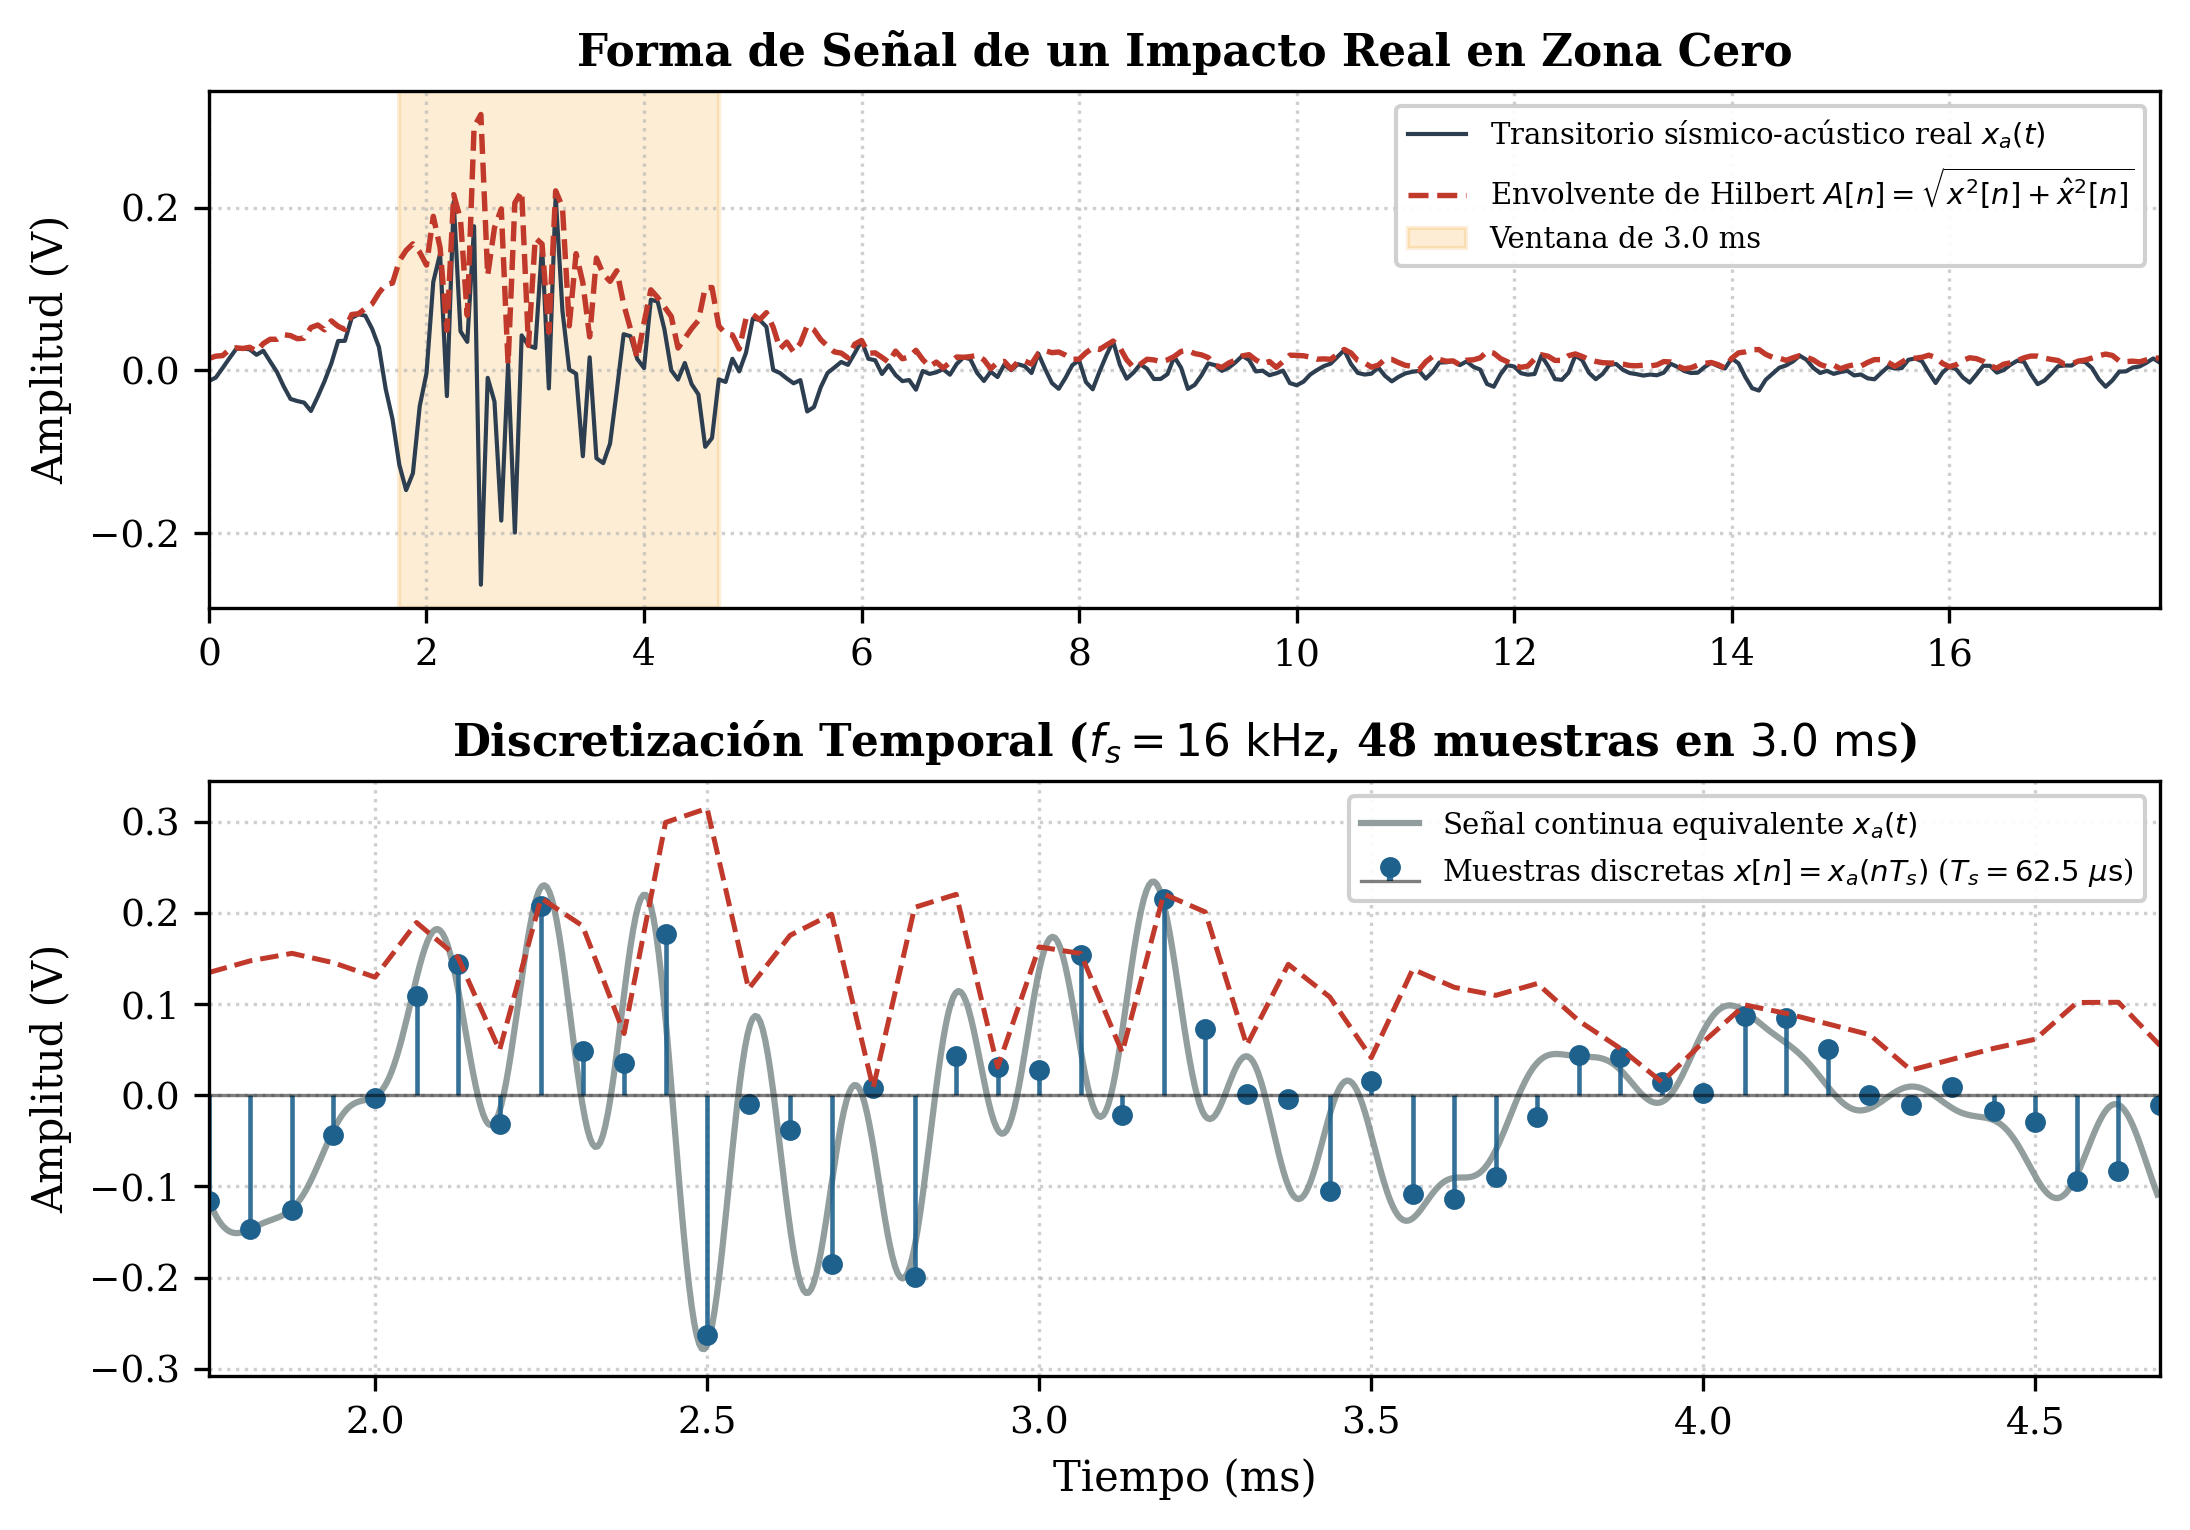
\includegraphics[width=0.45\textwidth]{../LaTex_figuras/fig1_impacto_real0.png}
    \caption{Señal analógica de impacto amortiguado $x_a(t)$ vs. secuencia muestreada discreta $x[n]$.}
    \label{fig:muestreo}
\end{figure}

Una vez discretizada la señal $x_a(t)$, se evaluó el comportamiento de los bloques Cuantificador (\textit{Quantizer}) y Codificador (\textit{Coder}) a 16 bits PCM, cuyos resultados se presentan en la Figura~\ref{fig:cuantificacion}. En la gráfica superior se observa que la secuencia cuantificada $x_q[n]$ se superpone sobre la señal en punto flotante $x[n]$ sin diferencias apreciables a simple vista, producto de los $65\,536$ niveles disponibles. Asimismo, en la gráfica inferior se inspeccionó la secuencia de error $e_q[n] = x_q[n] - x[n]$, comprobando que las variaciones se mantienen acotadas dentro de los límites teóricos $[-\Delta/2, +\Delta/2]$ ($\pm 1.52 \times 10^{-5}\text{ V}$ para $\Delta \approx 3.05 \times 10^{-5}\text{ V}$).

% --- ESPACIO PARA LA FIGURA 2 ---
\begin{figure}[htbp]
    \centering
    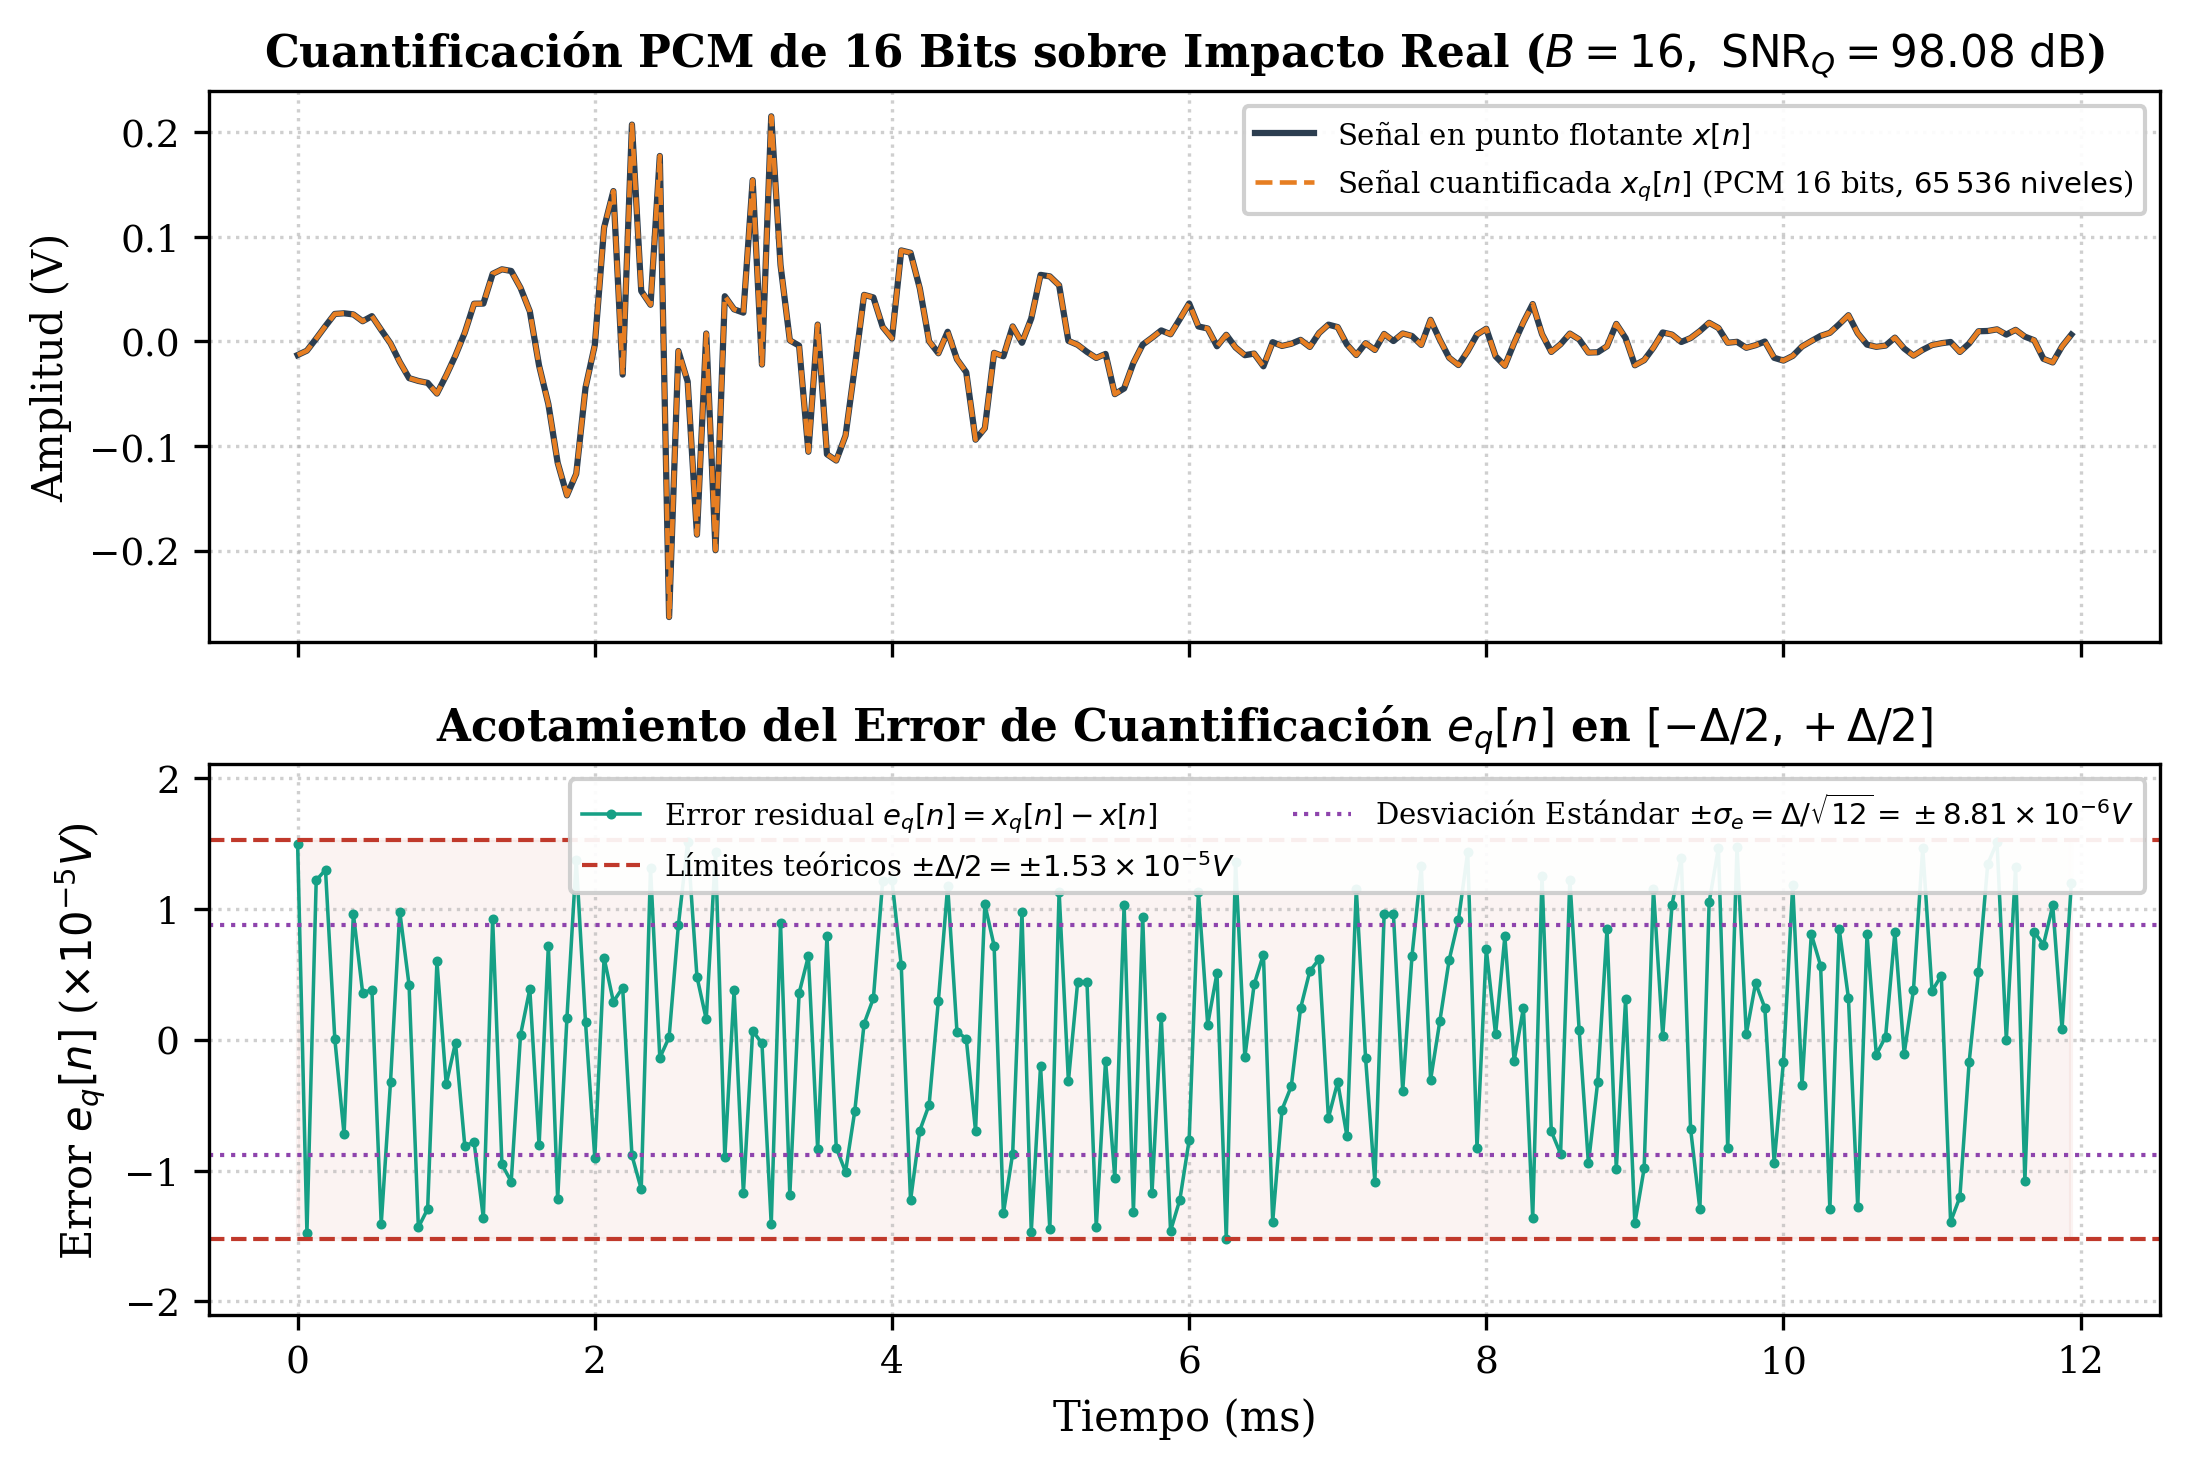
\includegraphics[width=0.45\textwidth]{../LaTex_figuras/fig2_cuantificacion.png}
    \caption{Arriba: Superposición de la señal analógica y cuantificada. Abajo: Vector de error de cuantificación $e_q[n]$.}
    \label{fig:cuantificacion}
\end{figure}

Finalmente, en la Figura~\ref{fig:filtrado} se validó el desempeño del filtrado IIR Butterworth de 4.º orden de fase cero comparando la señal cruda de terreno $x[n]$ frente a la señal acondicionada $y[n]$. En el panel superior se aprecia cómo la onda original se encuentra severamente distorsionada por una oscilación lenta de deriva de línea base ($<150\text{ Hz}$) y por ruido de alta frecuencia que ocultan los golpes de la víctima. Tras procesar el registro mediante el algoritmo bidireccional \texttt{filtfilt} en la banda de 150 a 7500 Hz (panel inferior), se logró eliminar la deriva estructural y estabilizar la línea base en cero, rescatando con claridad los picos transitorios del patrón rítmico y confirmando que estos coinciden exactamente con los instantes de impacto sin sufrir retardo de grupo ($\tau_g(\Omega) = 0$).

% --- ESPACIO PARA LA FIGURA 3 ---
\begin{figure}[htbp]
    \centering
    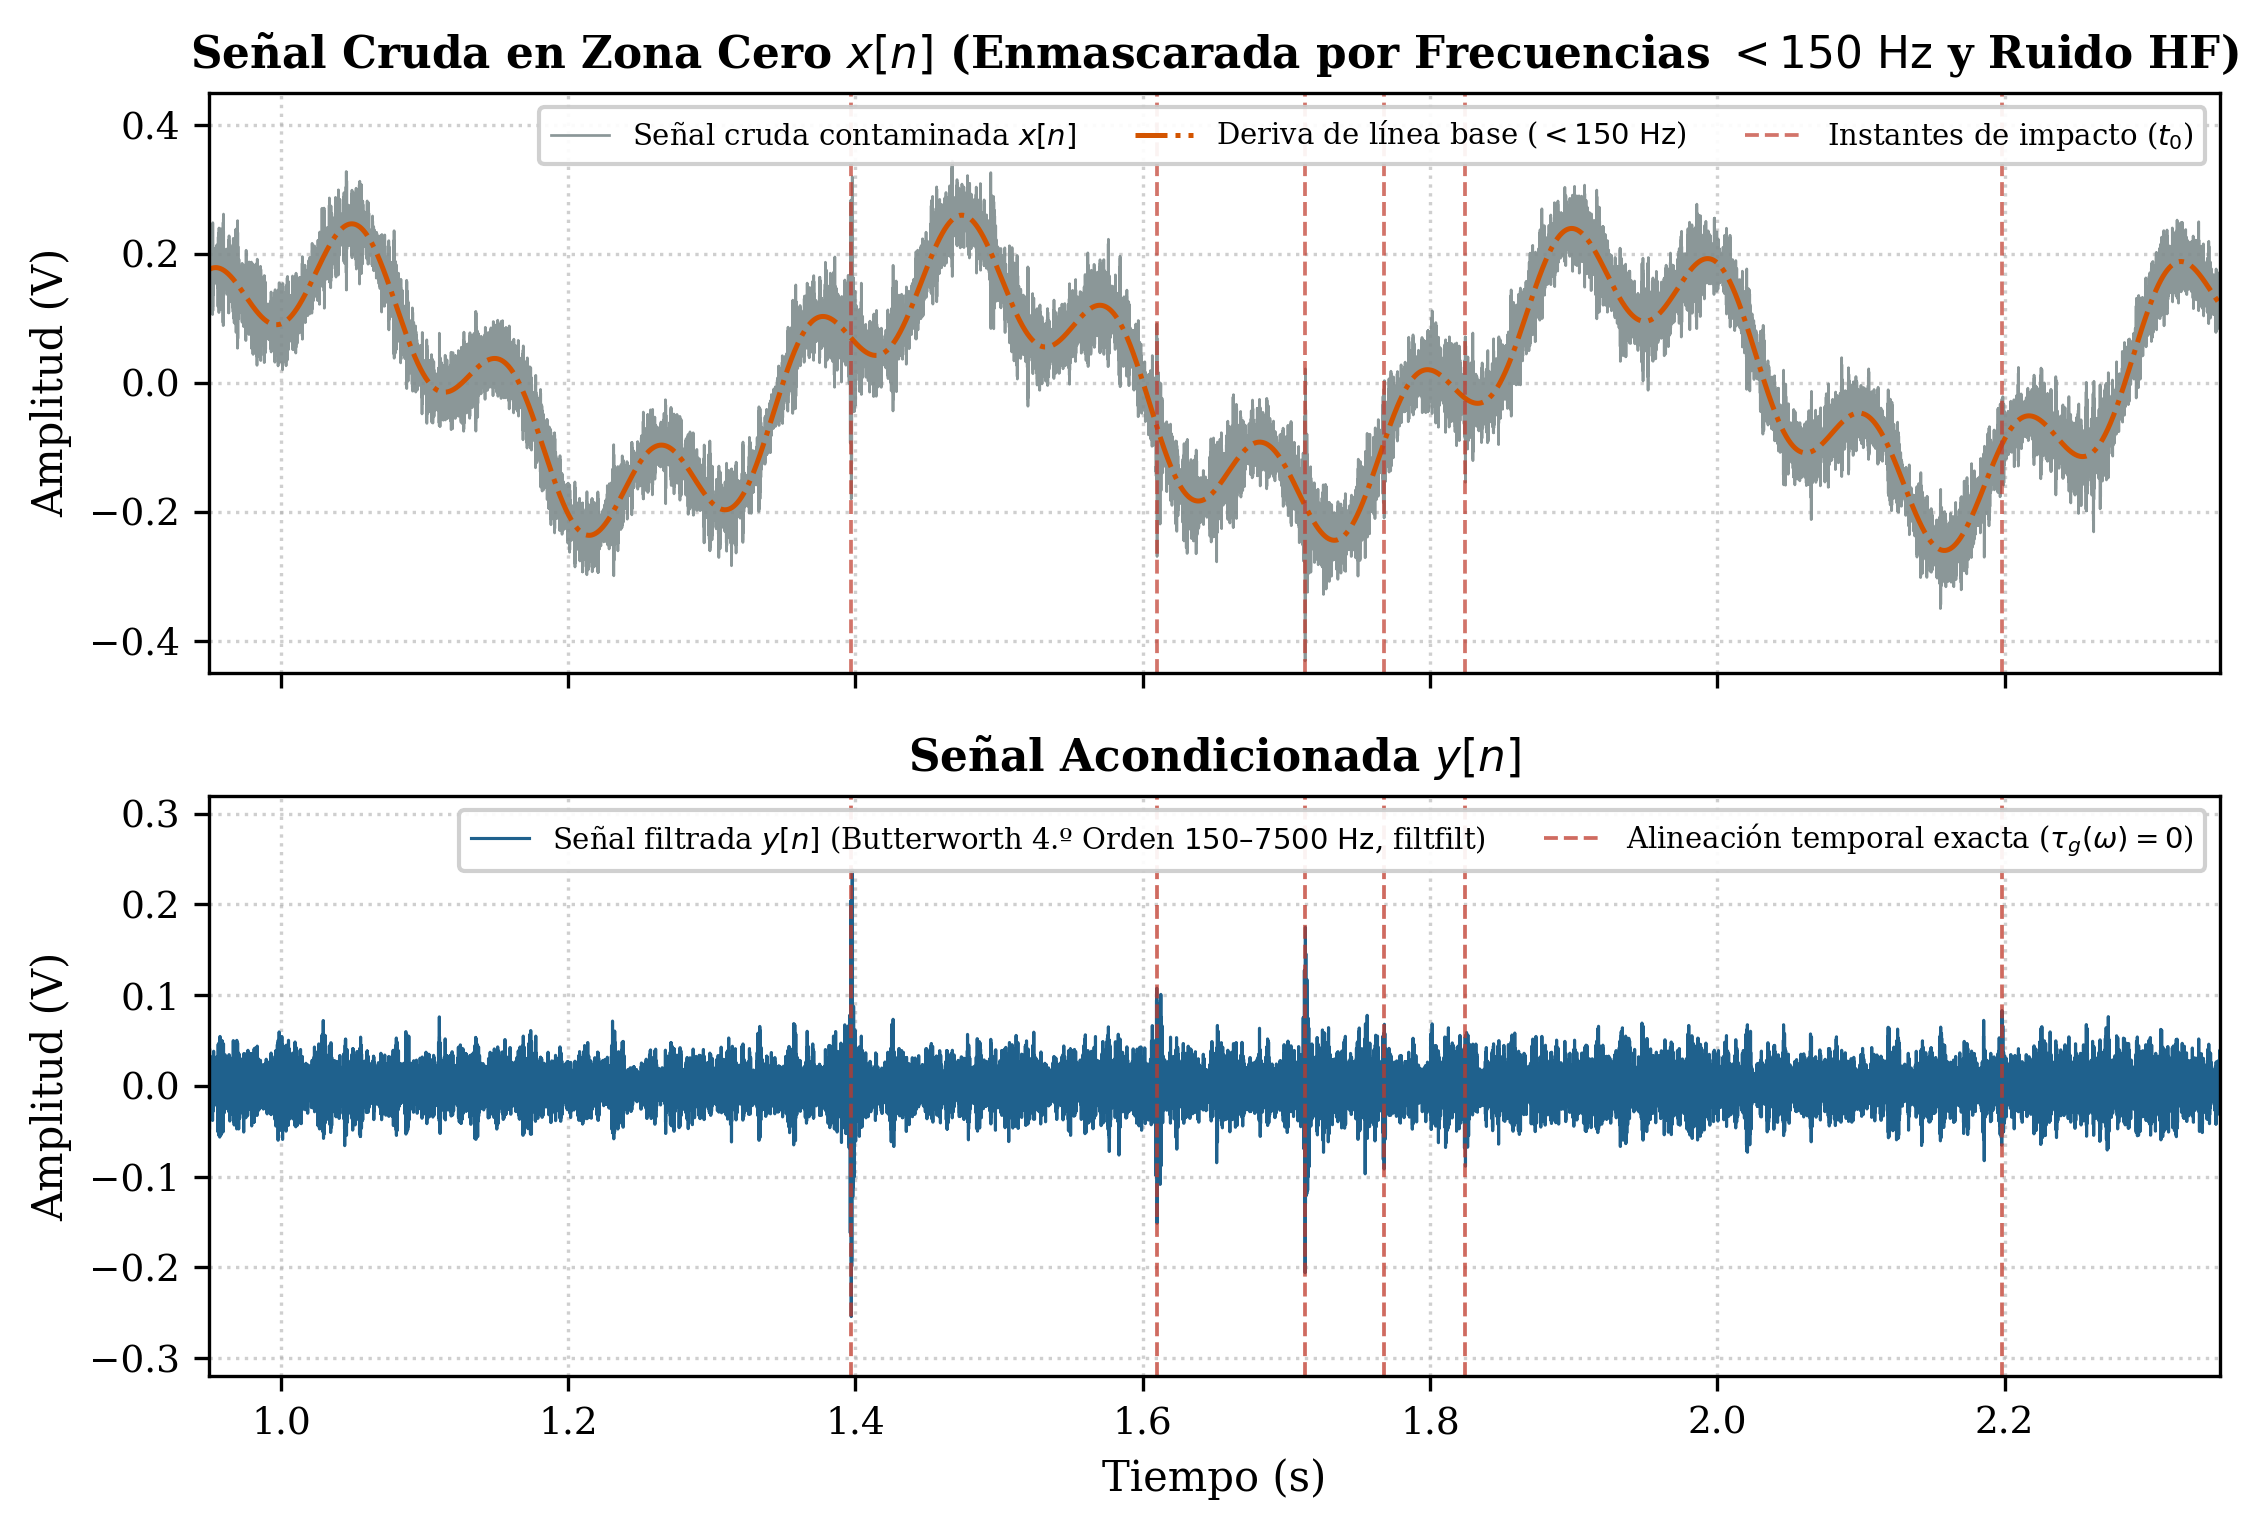
\includegraphics[width=0.45\textwidth]{../LaTex_figuras/fig3_filtrado_fase_cero_out.png}
    \caption{Comparativa espectro-temporal de la señal cruda con ruido de baja/alta frecuencia y la señal procesada $y[n]$.}
    \label{fig:filtrado}
\end{figure}

\section{Conclusiones}
El desarrollo de todos los objetivos planteados en este trabajo permitió estructurar y validar el pipeline de Procesamiento Digital de Señales para la detección pasiva de sobrevivientes en el sistema USAR V2.1. A partir de la caracterización de la señal sísmico-acústica y del diseño de la cadena de conversión A/D (\textit{Sampler}, \textit{Quantizer} y \textit{Coder}) operando a $f_s = 16\text{ kHz}$ y $16\text{ bits}$ PCM con ruido aditivo de \textit{dither}, se logró adquirir con fidelidad las micro-vibraciones en mampostería cumpliendo con el criterio de Nyquist-Shannon sin introducir solapamiento espectral (\textit{aliasing}) ni distorsión armónica \cite{Oppenheim, Proakis}. De igual manera, la implementación de ecuaciones en diferencias mediante el filtrado IIR Butterworth de 4.º orden con técnica bidireccional de fase cero (\texttt{filtfilt}) permitió suprimir la deriva de baja frecuencia y el ruido estructural manteniendo una respuesta de fase nula ($\phi_{\text{total}}(\Omega) = 0$), asegurando así la alineación temporal de los impactos de auxilio.

Asimismo, la extracción de la envolvente analítica mediante la Transformada de Hilbert y el motor de generación estocástica ($29\,953$ muestras rítmicas) proporcionaron las bases físicas para conformar e integrar un dataset consolidado y balanceado de $65\,576$ tensores, con el cual se entrenó y validó la arquitectura híbrida Convolucional Recurrente (CRNN \textit{Wide \& Deep}), alcanzando un F1-Score Macro de $0.8631$ y un ROC-AUC de $0.9927$. Todo esto se transformó en una herramienta computacional programada en Python y documentada bajo el estándar IEEE en \LaTeX{}, cumpliendo así con los requerimientos de sensibilidad, precisión temporal y confiabilidad operativa que exige la localización de vida en estructuras colapsadas.

\section*{Agradecimientos}
Se agradece el apoyo académico y técnico brindado por el profesor Gerlis Caropresse de la Universidad Central de Venezuela, al profesor Daniel Paredero del Instituto IMMUNE Technology, a las brigadas de rescate mexicanas Los Topos por la caracterización operativa del entorno y al equipo de HIKMICRO por la provisión de instrumentación acústica especializada (incluyendo el transductor piezoeléctrico de contacto AD21P y la cámara acústica AI56 para contraste superficial), cuyo aporte fue clave para la adquisición de datos de alta precisión y el desarrollo experimental de esta investigación.
% --- BIBLIOGRAFÍA ---
\begin{thebibliography}{9}
    \bibitem{Proakis}
    J. G. Proakis y D. G. Manolakis, \textit{Digital Signal Processing: Principles, Algorithms, and Applications}, 4ta ed. Upper Saddle River, NJ, EE. UU.: Pearson, 2006.
    
    \bibitem{Oppenheim}
    A. V. Oppenheim y R. W. Schafer, \textit{Discrete-Time Signal Processing}, 3ra ed. Upper Saddle River, NJ, EE. UU.: Prentice Hall, 2010.
\end{thebibliography}

\end{document}